\section{Datensatz}
\label{chap:datensatz}
Der Datensatz heißt \enquote{Stanford Dogs Dataset}\cite{datensatz} und besteht
aus 20580 Bildern von Hunden, die insgesamt 120 verschiedenen Rassen angehören.
Dabei entfallen auf jede Klasse ungefähr 150 Bilder, minimal 148 (Redbone) und
maximal 252 (Maltese Dog). Eine Übersicht mit Beispielbildern ist in
\autoref{fig:cluster} und eine Verteilung über die Anzahl der Bilder pro Rasse
in \autoref{fig:verteilung} dargestellt.

\begin{figure}
  \centering
  \includegraphics{pics/image_cluster.pdf}
  \caption{Zusammenstellung einiger Bilder aus dem Datensatz. Wie zu sehen ist,
  sind teilweise auch Menschen auf den Bildern zu sehen oder mehrere Hunde,
  was die Klassifikation erschwert.}
  \label{fig:cluster}
\end{figure}

\begin{figure}
  \centering
  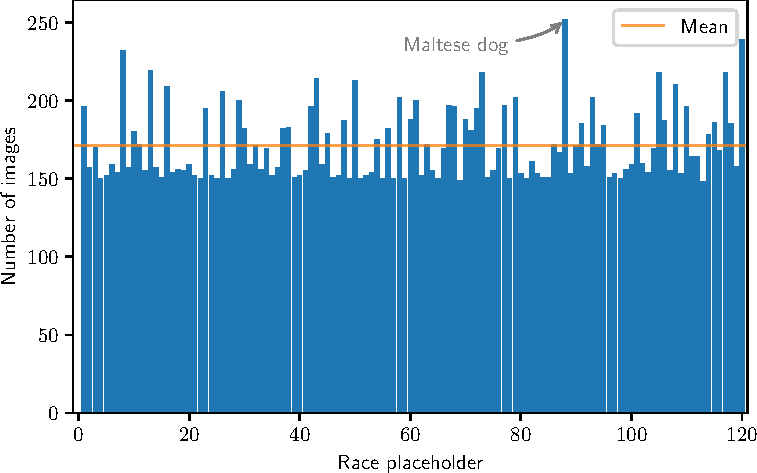
\includegraphics[scale=0.8]{pics/image_distribution.pdf}
  \caption{Anzahl der Bilder pro Rassen.}
  \label{fig:verteilung}
\end{figure}

Der Datensatz enthält neben den Klassenlabeln auch Bounding boxes, mit deren
Hilfe der Hund auf den Bildern identifiziert wird. Die Bilder sind keine
\enquote{biometrischen} Fotos von Hunden, da die Hunde teilweise nicht von vorne
abgelichtet sind, oder sich Menschen und/oder andere Tiere auf den Bildern
befinden, was die Klassifikation erschwert.

Aus dem großen Datensatz wurde ein kleinerer Datensatz mit nur fünf Klassen
erstellt, namentlich Chihuahua, Beagle, Schipperke, Standard Poodle und African
hunting dog, da im allgemeinen die Klassifikation besser funktioniert, wenn
weniger Klassen zur Auswahl stehen.
